\documentclass[a4paper]{book}
\usepackage{a4wide}
\usepackage{makeidx}
\usepackage{fancyhdr}
\usepackage{graphicx}
\usepackage{multicol}
\usepackage{float}
\usepackage{textcomp}
\usepackage{alltt}
\usepackage{times}
\usepackage{ifpdf}
\ifpdf
\usepackage[pdftex,
            pagebackref=true,
            colorlinks=true,
            linkcolor=blue
           ]{hyperref}
\else
\usepackage[ps2pdf,
            pagebackref=true,
            colorlinks=true,
            linkcolor=blue
           ]{hyperref}
\usepackage{pspicture}
\fi
\usepackage{doxygen}
\makeindex
\setcounter{tocdepth}{1}
\renewcommand{\footrulewidth}{0.4pt}
\begin{document}
\begin{titlepage}
\vspace*{7cm}
\begin{center}
{\Large Paradis\-EO-PEO - Lessons Reference Manual\\[1ex]\large 0.1 }\\
\vspace*{1cm}
{\large Generated by Doxygen 1.4.7}\\
\vspace*{0.5cm}
{\small Sun Jan 7 18:35:28 2007}\\
\end{center}
\end{titlepage}
\clearemptydoublepage
\pagenumbering{roman}
\tableofcontents
\clearemptydoublepage
\pagenumbering{arabic}
\chapter{Paradis\-EO-PEO - Lessons Hierarchical Index}
\section{Paradis\-EO-PEO Class Hierarchy}
This inheritance list is sorted roughly, but not completely, alphabetically:\begin{CompactList}
\item \contentsline{section}{Communicable}{\pageref{classCommunicable}}{}
\begin{CompactList}
\item \contentsline{section}{Cooperative}{\pageref{classCooperative}}{}
\begin{CompactList}
\item \contentsline{section}{peo\-Async\-Island\-Mig$<$ EOT $>$}{\pageref{classpeoAsyncIslandMig}}{}
\item \contentsline{section}{peo\-Sync\-Island\-Mig$<$ EOT $>$}{\pageref{classpeoSyncIslandMig}}{}
\end{CompactList}
\item \contentsline{section}{Runner}{\pageref{classRunner}}{}
\begin{CompactList}
\item \contentsline{section}{peo\-EA$<$ EOT $>$}{\pageref{classpeoEA}}{}
\end{CompactList}
\item \contentsline{section}{Service}{\pageref{classService}}{}
\begin{CompactList}
\item \contentsline{section}{peo\-Pop\-Eval$<$ EOT $>$}{\pageref{classpeoPopEval}}{}
\begin{CompactList}
\item \contentsline{section}{peo\-Para\-Pop\-Eval$<$ EOT $>$}{\pageref{classpeoParaPopEval}}{}
\item \contentsline{section}{peo\-Seq\-Pop\-Eval$<$ EOT $>$}{\pageref{classpeoSeqPopEval}}{}
\end{CompactList}
\item \contentsline{section}{peo\-Sync\-Multi\-Start$<$ EOT $>$}{\pageref{classpeoSyncMultiStart}}{}
\item \contentsline{section}{peo\-Transform$<$ EOT $>$}{\pageref{classpeoTransform}}{}
\begin{CompactList}
\item \contentsline{section}{peo\-Para\-SGATransform$<$ EOT $>$}{\pageref{classpeoParaSGATransform}}{}
\item \contentsline{section}{peo\-Seq\-Transform$<$ EOT $>$}{\pageref{classpeoSeqTransform}}{}
\end{CompactList}
\end{CompactList}
\item \contentsline{section}{Worker}{\pageref{classWorker}}{}
\end{CompactList}
\item eo\-Functor\-Base{\tt  \mbox{[}external\mbox{]}}\begin{CompactList}
\item eo\-BF$<$ A1, A2, R $>${\tt  \mbox{[}external\mbox{]}}\begin{CompactList}
\item \contentsline{section}{peo\-Agg\-Eval\-Func$<$ EOT $>$}{\pageref{classpeoAggEvalFunc}}{}
\begin{CompactList}
\item \contentsline{section}{peo\-No\-Agg\-Eval\-Func$<$ EOT $>$}{\pageref{classpeoNoAggEvalFunc}}{}
\end{CompactList}
\end{CompactList}
\item eo\-F$<$ void $>${\tt  \mbox{[}external\mbox{]}}\begin{CompactList}
\item eo\-Updater{\tt  \mbox{[}external\mbox{]}}\begin{CompactList}
\item \contentsline{section}{peo\-Async\-Island\-Mig$<$ EOT $>$}{\pageref{classpeoAsyncIslandMig}}{}
\item \contentsline{section}{peo\-Sync\-Island\-Mig$<$ EOT $>$}{\pageref{classpeoSyncIslandMig}}{}
\item \contentsline{section}{peo\-Sync\-Multi\-Start$<$ EOT $>$}{\pageref{classpeoSyncMultiStart}}{}
\end{CompactList}
\end{CompactList}
\item eo\-UF$<$ A1, R $>${\tt  \mbox{[}external\mbox{]}}\begin{CompactList}
\item eo\-Transform$<$ EOT $>${\tt  \mbox{[}external\mbox{]}}\begin{CompactList}
\item \contentsline{section}{peo\-Transform$<$ EOT $>$}{\pageref{classpeoTransform}}{}
\end{CompactList}
\end{CompactList}
\end{CompactList}
\item \contentsline{section}{SEND\_\-REQUEST}{\pageref{structSEND__REQUEST}}{}
\item \contentsline{section}{Thread}{\pageref{classThread}}{}
\begin{CompactList}
\item \contentsline{section}{Reactive\-Thread}{\pageref{classReactiveThread}}{}
\begin{CompactList}
\item \contentsline{section}{Communicator}{\pageref{classCommunicator}}{}
\item \contentsline{section}{Worker}{\pageref{classWorker}}{}
\end{CompactList}
\item \contentsline{section}{Runner}{\pageref{classRunner}}{}
\end{CompactList}
\item \contentsline{section}{Topology}{\pageref{classTopology}}{}
\begin{CompactList}
\item \contentsline{section}{Ring\-Topology}{\pageref{classRingTopology}}{}
\end{CompactList}
\end{CompactList}

\chapter{Paradis\-EO-PEO - Lessons Class Index}
\section{Paradis\-EO Class List}
Here are the classes, structs, unions and interfaces with brief descriptions:\begin{CompactList}
\item\contentsline{section}{\bf{City\-Swap} (Its swaps two vertices randomly choosen )}{\pageref{class_city_swap}}{}
\item\contentsline{section}{\bf{Communicable} }{\pageref{class_communicable}}{}
\item\contentsline{section}{\bf{Communicator} }{\pageref{class_communicator}}{}
\item\contentsline{section}{\bf{Cooperative} }{\pageref{class_cooperative}}{}
\item\contentsline{section}{\bf{Display\-Best\-Route} }{\pageref{class_display_best_route}}{}
\item\contentsline{section}{\bf{Edge\-Xover} (Edge Crossover )}{\pageref{class_edge_xover}}{}
\item\contentsline{section}{\bf{Merge\-Route\-Eval} }{\pageref{class_merge_route_eval}}{}
\item\contentsline{section}{\bf{Node} }{\pageref{struct_node}}{}
\item\contentsline{section}{\bf{Order\-Xover} (Order Crossover )}{\pageref{class_order_xover}}{}
\item\contentsline{section}{\bf{Partial\-Mapped\-Xover} (Partial Mapped Crossover )}{\pageref{class_partial_mapped_xover}}{}
\item\contentsline{section}{\bf{Part\-Route\-Eval} (Route Evaluator )}{\pageref{class_part_route_eval}}{}
\item\contentsline{section}{\bf{peo\-Agg\-Eval\-Func$<$ EOT $>$} (The \doxyref{peo\-Agg\-Eval\-Func}{p.}{classpeo_agg_eval_func} class offers only the interface for creating aggregate evaluation functions - there are no direct internal functions provided )}{\pageref{classpeo_agg_eval_func}}{}
\item\contentsline{section}{\bf{peo\-Async\-Island\-Mig$<$ EOT $>$} (The \doxyref{peo\-Async\-Island\-Mig}{p.}{classpeo_async_island_mig} class offers the elementary basis for implementating an asynchronous island migration model - requires the specification of several basic parameters, i.e )}{\pageref{classpeo_async_island_mig}}{}
\item\contentsline{section}{\bf{peo\-EA$<$ EOT $>$} (The \doxyref{peo\-EA}{p.}{classpeo_e_a} class offers an elementary evolutionary algorithm implementation )}{\pageref{classpeo_e_a}}{}
\item\contentsline{section}{\bf{peo\-No\-Agg\-Eval\-Func$<$ EOT $>$} (The \doxyref{peo\-No\-Agg\-Eval\-Func}{p.}{classpeo_no_agg_eval_func} class does nothing more than an association between a fitness value and a specified individual )}{\pageref{classpeo_no_agg_eval_func}}{}
\item\contentsline{section}{\bf{peo\-Para\-Pop\-Eval$<$ EOT $>$} (The \doxyref{peo\-Para\-Pop\-Eval}{p.}{classpeo_para_pop_eval} represents a wrapper for creating a functor capable of applying in parallel an EO-derived evaluation functor )}{\pageref{classpeo_para_pop_eval}}{}
\item\contentsline{section}{\bf{peo\-Para\-SGATransform$<$ EOT $>$} }{\pageref{classpeo_para_s_g_a_transform}}{}
\item\contentsline{section}{\bf{peo\-Pop\-Eval$<$ EOT $>$} (The {\bf \doxyref{peo\-Pop\-Eval}{p.}{classpeo_pop_eval}} class provides the interface for constructing Paradis\-EO specific evaluation functors )}{\pageref{classpeo_pop_eval}}{}
\item\contentsline{section}{\bf{peo\-Seq\-Pop\-Eval$<$ EOT $>$} (The \doxyref{peo\-Seq\-Pop\-Eval}{p.}{classpeo_seq_pop_eval} class acts only as a Paradis\-EO specific sequential evaluation functor - a wrapper for incorporating an {\bf eo\-Eval\-Func$<$ EOT $>$}-derived class as evaluation functor )}{\pageref{classpeo_seq_pop_eval}}{}
\item\contentsline{section}{\bf{peo\-Seq\-Transform$<$ EOT $>$} (The \doxyref{peo\-Seq\-Transform}{p.}{classpeo_seq_transform} represent a wrapper for offering the possibility of using EO derived transform operators along with the Paradis\-EO evolutionary algorithms )}{\pageref{classpeo_seq_transform}}{}
\item\contentsline{section}{\bf{peo\-Sync\-Island\-Mig$<$ EOT $>$} (The \doxyref{peo\-Sync\-Island\-Mig}{p.}{classpeo_sync_island_mig} class offers the elementary basis for implementating a synchronous island migration model - requires the specification of several basic parameters, i.e )}{\pageref{classpeo_sync_island_mig}}{}
\item\contentsline{section}{\bf{peo\-Sync\-Multi\-Start$<$ EOT $>$} (The \doxyref{peo\-Sync\-Multi\-Start}{p.}{classpeo_sync_multi_start} class provides the basis for implementing the synchronous multi-start model, for launching several solution-based algorithms in parallel on a specified initial population )}{\pageref{classpeo_sync_multi_start}}{}
\item\contentsline{section}{\bf{peo\-Transform$<$ EOT $>$} (The \doxyref{peo\-Transform}{p.}{classpeo_transform} class acts only as an interface for creating transform operators - for an example please refer to the {\bf \doxyref{peo\-Seq\-Transform}{p.}{classpeo_seq_transform}} and the {\bf \doxyref{peo\-Para\-SGATransform}{p.}{classpeo_para_s_g_a_transform}} classes )}{\pageref{classpeo_transform}}{}
\item\contentsline{section}{\bf{Reactive\-Thread} }{\pageref{class_reactive_thread}}{}
\item\contentsline{section}{\bf{Ring\-Topology} }{\pageref{class_ring_topology}}{}
\item\contentsline{section}{\bf{Route\-Eval} }{\pageref{class_route_eval}}{}
\item\contentsline{section}{\bf{Route\-Init} }{\pageref{class_route_init}}{}
\item\contentsline{section}{\bf{Runner} }{\pageref{class_runner}}{}
\item\contentsline{section}{\bf{SEND\_\-REQUEST} }{\pageref{struct_s_e_n_d___r_e_q_u_e_s_t}}{}
\item\contentsline{section}{\bf{Service} }{\pageref{class_service}}{}
\item\contentsline{section}{\bf{Thread} }{\pageref{class_thread}}{}
\item\contentsline{section}{\bf{Topology} }{\pageref{class_topology}}{}
\item\contentsline{section}{\bf{Two\-Opt} }{\pageref{class_two_opt}}{}
\item\contentsline{section}{\bf{Two\-Opt\-Incr\-Eval} }{\pageref{class_two_opt_incr_eval}}{}
\item\contentsline{section}{\bf{Two\-Opt\-Init} }{\pageref{class_two_opt_init}}{}
\item\contentsline{section}{\bf{Two\-Opt\-Next} }{\pageref{class_two_opt_next}}{}
\item\contentsline{section}{\bf{Two\-Opt\-Rand} }{\pageref{class_two_opt_rand}}{}
\item\contentsline{section}{\bf{Worker} }{\pageref{class_worker}}{}
\end{CompactList}

\chapter{Paradis\-EO-PEO - Lessons Class Documentation}
\hypertarget{classCitySwap}{
\section{City\-Swap Class Reference}
\label{classCitySwap}\index{CitySwap@{CitySwap}}
}
Its swaps two vertices randomly choosen.  


{\tt \#include $<$city\_\-swap.h$>$}

\subsection*{Public Member Functions}
\begin{CompactItemize}
\item 
\hypertarget{classCitySwap_7e6958b62048c89604cbf046b86bdf2d}{
bool \hyperlink{classCitySwap_7e6958b62048c89604cbf046b86bdf2d}{operator()} (Route \&\_\-\_\-route)}
\label{classCitySwap_7e6958b62048c89604cbf046b86bdf2d}

\end{CompactItemize}


\subsection{Detailed Description}
Its swaps two vertices randomly choosen. 



Definition at line 33 of file city\_\-swap.h.

The documentation for this class was generated from the following files:\begin{CompactItemize}
\item 
city\_\-swap.h\item 
city\_\-swap.cpp\end{CompactItemize}

\hypertarget{classDisplayBestRoute}{
\section{Display\-Best\-Route Class Reference}
\label{classDisplayBestRoute}\index{DisplayBestRoute@{DisplayBestRoute}}
}
Inheritance diagram for Display\-Best\-Route::\begin{figure}[H]
\begin{center}
\leavevmode
\includegraphics[height=4cm]{classDisplayBestRoute}
\end{center}
\end{figure}
\subsection*{Public Member Functions}
\begin{CompactItemize}
\item 
\hypertarget{classDisplayBestRoute_db263e38f1e82174f811bf62f323f87f}{
\hyperlink{classDisplayBestRoute_db263e38f1e82174f811bf62f323f87f}{Display\-Best\-Route} (\bf{eo\-Pop}$<$ \bf{Route} $>$ \&\_\-\_\-pop)}
\label{classDisplayBestRoute_db263e38f1e82174f811bf62f323f87f}

\item 
\hypertarget{classDisplayBestRoute_ee879344a6d8b81a04d4eabbed2c7a04}{
void \hyperlink{classDisplayBestRoute_ee879344a6d8b81a04d4eabbed2c7a04}{operator()} ()}
\label{classDisplayBestRoute_ee879344a6d8b81a04d4eabbed2c7a04}

\end{CompactItemize}
\subsection*{Private Attributes}
\begin{CompactItemize}
\item 
\hypertarget{classDisplayBestRoute_5270aabbf294d2deca9878934216eb89}{
\bf{eo\-Pop}$<$ \bf{Route} $>$ \& \hyperlink{classDisplayBestRoute_5270aabbf294d2deca9878934216eb89}{pop}}
\label{classDisplayBestRoute_5270aabbf294d2deca9878934216eb89}

\end{CompactItemize}


\subsection{Detailed Description}




Definition at line 46 of file display\_\-best\_\-route.h.

The documentation for this class was generated from the following files:\begin{CompactItemize}
\item 
display\_\-best\_\-route.h\item 
display\_\-best\_\-route.cpp\end{CompactItemize}

\hypertarget{classEdgeXover}{
\section{Edge\-Xover Class Reference}
\label{classEdgeXover}\index{EdgeXover@{EdgeXover}}
}
Edge Crossover.  


{\tt \#include $<$edge\_\-xover.h$>$}

\subsection*{Public Member Functions}
\begin{CompactItemize}
\item 
\hypertarget{classEdgeXover_cb1c0a103106a4d3319540cb23163a79}{
bool \hyperlink{classEdgeXover_cb1c0a103106a4d3319540cb23163a79}{operator()} (Route \&\_\-\_\-route1, Route \&\_\-\_\-route2)}
\label{classEdgeXover_cb1c0a103106a4d3319540cb23163a79}

\end{CompactItemize}
\subsection*{Private Member Functions}
\begin{CompactItemize}
\item 
\hypertarget{classEdgeXover_88c2d4c9a878454a32d56010f3dddc27}{
void \hyperlink{classEdgeXover_88c2d4c9a878454a32d56010f3dddc27}{cross} (const Route \&\_\-\_\-par1, const Route \&\_\-\_\-par2, Route \&\_\-\_\-child)}
\label{classEdgeXover_88c2d4c9a878454a32d56010f3dddc27}

\item 
\hypertarget{classEdgeXover_1b3a4c75dd9a034c81af6d89d85d30f5}{
void \hyperlink{classEdgeXover_1b3a4c75dd9a034c81af6d89d85d30f5}{remove\_\-entry} (unsigned \_\-\_\-vertex, std::vector$<$ std::set$<$ unsigned $>$ $>$ \&\_\-\_\-map)}
\label{classEdgeXover_1b3a4c75dd9a034c81af6d89d85d30f5}

\item 
\hypertarget{classEdgeXover_04de96aa1016836e0ba5f4b952a5fa16}{
void \hyperlink{classEdgeXover_04de96aa1016836e0ba5f4b952a5fa16}{build\_\-map} (const Route \&\_\-\_\-par1, const Route \&\_\-\_\-par2)}
\label{classEdgeXover_04de96aa1016836e0ba5f4b952a5fa16}

\item 
\hypertarget{classEdgeXover_2d3045ef503d8b16a27e11fdc23ca11c}{
void \hyperlink{classEdgeXover_2d3045ef503d8b16a27e11fdc23ca11c}{add\_\-vertex} (unsigned \_\-\_\-vertex, Route \&\_\-\_\-child)}
\label{classEdgeXover_2d3045ef503d8b16a27e11fdc23ca11c}

\end{CompactItemize}
\subsection*{Private Attributes}
\begin{CompactItemize}
\item 
\hypertarget{classEdgeXover_d41399c6effb54ee48c722f1e19cb3c3}{
std::vector$<$ std::set$<$ unsigned $>$ $>$ \hyperlink{classEdgeXover_d41399c6effb54ee48c722f1e19cb3c3}{\_\-map}}
\label{classEdgeXover_d41399c6effb54ee48c722f1e19cb3c3}

\item 
\hypertarget{classEdgeXover_46d4d4724cf6d660b1a7ab4a346573d4}{
std::vector$<$ bool $>$ \hyperlink{classEdgeXover_46d4d4724cf6d660b1a7ab4a346573d4}{visited}}
\label{classEdgeXover_46d4d4724cf6d660b1a7ab4a346573d4}

\end{CompactItemize}


\subsection{Detailed Description}
Edge Crossover. 



Definition at line 35 of file edge\_\-xover.h.

The documentation for this class was generated from the following files:\begin{CompactItemize}
\item 
edge\_\-xover.h\item 
edge\_\-xover.cpp\end{CompactItemize}

\hypertarget{classMergeRouteEval}{
\section{Merge\-Route\-Eval Class Reference}
\label{classMergeRouteEval}\index{MergeRouteEval@{MergeRouteEval}}
}
Inheritance diagram for Merge\-Route\-Eval::\begin{figure}[H]
\begin{center}
\leavevmode
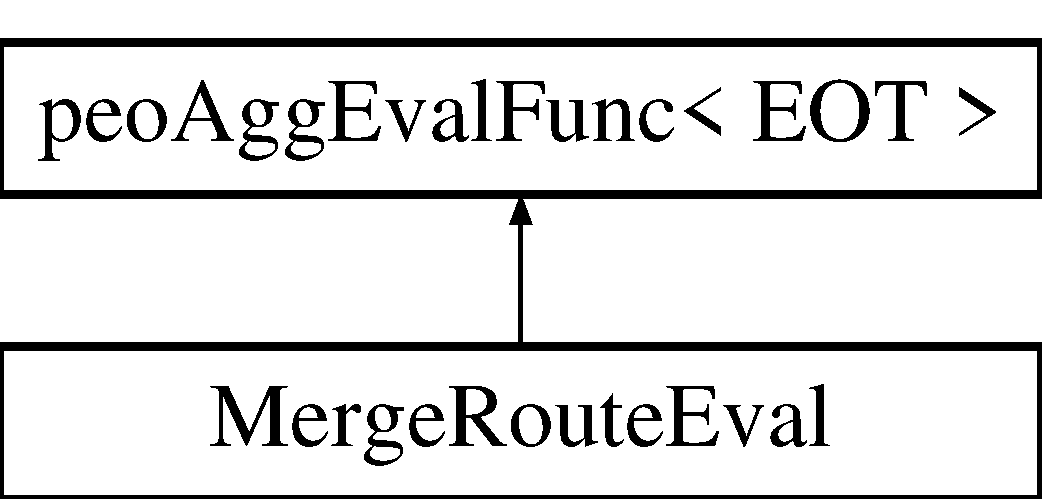
\includegraphics[height=2cm]{classMergeRouteEval}
\end{center}
\end{figure}
\subsection*{Public Member Functions}
\begin{CompactItemize}
\item 
\hypertarget{classMergeRouteEval_29cb0028ac0df4b2cee3a809c8f35dea}{
void \hyperlink{classMergeRouteEval_29cb0028ac0df4b2cee3a809c8f35dea}{operator()} (Route \&\_\-\_\-route, const int \&\_\-\_\-part\_\-fit)}
\label{classMergeRouteEval_29cb0028ac0df4b2cee3a809c8f35dea}

\end{CompactItemize}


\subsection{Detailed Description}




Definition at line 31 of file merge\_\-route\_\-eval.h.

The documentation for this class was generated from the following files:\begin{CompactItemize}
\item 
merge\_\-route\_\-eval.h\item 
merge\_\-route\_\-eval.cpp\end{CompactItemize}

\hypertarget{classOrderXover}{
\section{Order\-Xover Class Reference}
\label{classOrderXover}\index{OrderXover@{OrderXover}}
}
Order Crossover.  


{\tt \#include $<$order\_\-xover.h$>$}

\subsection*{Public Member Functions}
\begin{CompactItemize}
\item 
\hypertarget{classOrderXover_0ff6aada669eb8173322ed68cda1ac61}{
bool \hyperlink{classOrderXover_0ff6aada669eb8173322ed68cda1ac61}{operator()} (Route \&\_\-\_\-route1, Route \&\_\-\_\-route2)}
\label{classOrderXover_0ff6aada669eb8173322ed68cda1ac61}

\end{CompactItemize}
\subsection*{Private Member Functions}
\begin{CompactItemize}
\item 
\hypertarget{classOrderXover_d2bf90b5f46ac4a344777e17bc5f364d}{
void \hyperlink{classOrderXover_d2bf90b5f46ac4a344777e17bc5f364d}{cross} (const Route \&\_\-\_\-par1, const Route \&\_\-\_\-par2, Route \&\_\-\_\-child)}
\label{classOrderXover_d2bf90b5f46ac4a344777e17bc5f364d}

\end{CompactItemize}


\subsection{Detailed Description}
Order Crossover. 



Definition at line 17 of file order\_\-xover.h.

The documentation for this class was generated from the following files:\begin{CompactItemize}
\item 
order\_\-xover.h\item 
order\_\-xover.cpp\end{CompactItemize}

\hypertarget{classPartialMappedXover}{
\section{Partial\-Mapped\-Xover Class Reference}
\label{classPartialMappedXover}\index{PartialMappedXover@{PartialMappedXover}}
}
Partial Mapped Crossover.  


{\tt \#include $<$partial\_\-mapped\_\-xover.h$>$}

\subsection*{Public Member Functions}
\begin{CompactItemize}
\item 
\hypertarget{classPartialMappedXover_1cda6ea86ca36e5de0125f4ba5cfc695}{
bool \hyperlink{classPartialMappedXover_1cda6ea86ca36e5de0125f4ba5cfc695}{operator()} (Route \&\_\-\_\-route1, Route \&\_\-\_\-route2)}
\label{classPartialMappedXover_1cda6ea86ca36e5de0125f4ba5cfc695}

\end{CompactItemize}
\subsection*{Private Member Functions}
\begin{CompactItemize}
\item 
\hypertarget{classPartialMappedXover_b6d4035544aff3b2b3fe4b0eeea185a2}{
void \hyperlink{classPartialMappedXover_b6d4035544aff3b2b3fe4b0eeea185a2}{repair} (Route \&\_\-\_\-route, unsigned \_\-\_\-cut1, unsigned \_\-\_\-cut2)}
\label{classPartialMappedXover_b6d4035544aff3b2b3fe4b0eeea185a2}

\end{CompactItemize}


\subsection{Detailed Description}
Partial Mapped Crossover. 



Definition at line 17 of file partial\_\-mapped\_\-xover.h.

The documentation for this class was generated from the following files:\begin{CompactItemize}
\item 
partial\_\-mapped\_\-xover.h\item 
partial\_\-mapped\_\-xover.cpp\end{CompactItemize}

\hypertarget{classPartRouteEval}{
\section{Part\-Route\-Eval Class Reference}
\label{classPartRouteEval}\index{PartRouteEval@{PartRouteEval}}
}
Route Evaluator.  


{\tt \#include $<$part\_\-route\_\-eval.h$>$}

\subsection*{Public Member Functions}
\begin{CompactItemize}
\item 
\hypertarget{classPartRouteEval_a331566b29bc3227f377004232f05491}{
\hyperlink{classPartRouteEval_a331566b29bc3227f377004232f05491}{Part\-Route\-Eval} (float \_\-\_\-from, float \_\-\_\-to)}
\label{classPartRouteEval_a331566b29bc3227f377004232f05491}

\begin{CompactList}\small\item\em Constructor. \item\end{CompactList}\item 
\hypertarget{classPartRouteEval_965fab875fb601f17934a6ece761beae}{
void \hyperlink{classPartRouteEval_965fab875fb601f17934a6ece761beae}{operator()} (Route \&\_\-\_\-route)}
\label{classPartRouteEval_965fab875fb601f17934a6ece761beae}

\end{CompactItemize}
\subsection*{Private Attributes}
\begin{CompactItemize}
\item 
\hypertarget{classPartRouteEval_5bde722e66378b2570ae6c4b4f8df58e}{
float \hyperlink{classPartRouteEval_5bde722e66378b2570ae6c4b4f8df58e}{from}}
\label{classPartRouteEval_5bde722e66378b2570ae6c4b4f8df58e}

\item 
\hypertarget{classPartRouteEval_de53cc919faa498663f327b72c357da3}{
float \hyperlink{classPartRouteEval_de53cc919faa498663f327b72c357da3}{to}}
\label{classPartRouteEval_de53cc919faa498663f327b72c357da3}

\end{CompactItemize}


\subsection{Detailed Description}
Route Evaluator. 



Definition at line 32 of file part\_\-route\_\-eval.h.

The documentation for this class was generated from the following files:\begin{CompactItemize}
\item 
part\_\-route\_\-eval.h\item 
part\_\-route\_\-eval.cpp\end{CompactItemize}

\hypertarget{classRouteEval}{
\section{Route\-Eval Class Reference}
\label{classRouteEval}\index{RouteEval@{RouteEval}}
}
\subsection*{Public Member Functions}
\begin{CompactItemize}
\item 
\hypertarget{classRouteEval_e10bbe6f792e6f44405953de4f703901}{
void \hyperlink{classRouteEval_e10bbe6f792e6f44405953de4f703901}{operator()} (Route \&\_\-\_\-route)}
\label{classRouteEval_e10bbe6f792e6f44405953de4f703901}

\end{CompactItemize}


\subsection{Detailed Description}




Definition at line 31 of file route\_\-eval.h.

The documentation for this class was generated from the following files:\begin{CompactItemize}
\item 
route\_\-eval.h\item 
route\_\-eval.cpp\end{CompactItemize}

\hypertarget{classRouteInit}{
\section{Route\-Init Class Reference}
\label{classRouteInit}\index{RouteInit@{RouteInit}}
}
\subsection*{Public Member Functions}
\begin{CompactItemize}
\item 
\hypertarget{classRouteInit_b65a7137e114458faadb6a5510c001f7}{
void \hyperlink{classRouteInit_b65a7137e114458faadb6a5510c001f7}{operator()} (Route \&\_\-\_\-route)}
\label{classRouteInit_b65a7137e114458faadb6a5510c001f7}

\end{CompactItemize}


\subsection{Detailed Description}




Definition at line 31 of file route\_\-init.h.

The documentation for this class was generated from the following files:\begin{CompactItemize}
\item 
route\_\-init.h\item 
route\_\-init.cpp\end{CompactItemize}

\hypertarget{classTwoOpt}{
\section{Two\-Opt Class Reference}
\label{classTwoOpt}\index{TwoOpt@{TwoOpt}}
}
Inheritance diagram for Two\-Opt::\begin{figure}[H]
\begin{center}
\leavevmode
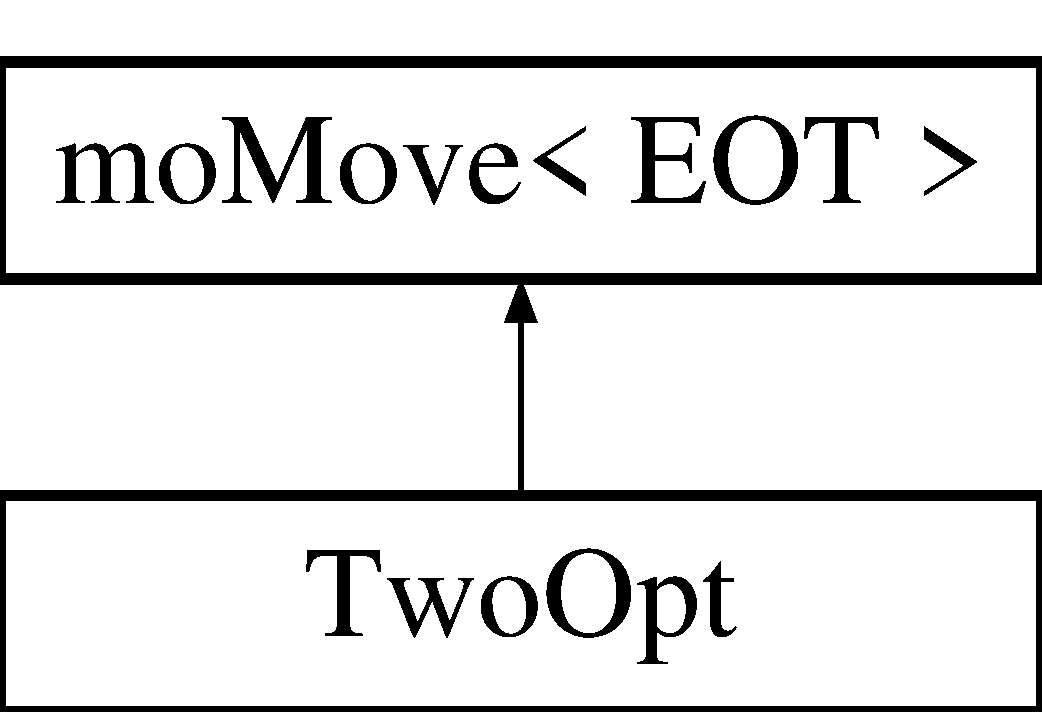
\includegraphics[height=2cm]{classTwoOpt}
\end{center}
\end{figure}
\subsection*{Public Member Functions}
\begin{CompactItemize}
\item 
\hypertarget{classTwoOpt_ff87d1649a33d42a6d64e8d314ed1af0}{
void \hyperlink{classTwoOpt_ff87d1649a33d42a6d64e8d314ed1af0}{operator()} (Route \&\_\-\_\-route)}
\label{classTwoOpt_ff87d1649a33d42a6d64e8d314ed1af0}

\end{CompactItemize}


\subsection{Detailed Description}




Definition at line 32 of file two\_\-opt.h.

The documentation for this class was generated from the following files:\begin{CompactItemize}
\item 
two\_\-opt.h\item 
two\_\-opt.cpp\end{CompactItemize}

\hypertarget{classTwoOptIncrEval}{
\section{Two\-Opt\-Incr\-Eval Class Reference}
\label{classTwoOptIncrEval}\index{TwoOptIncrEval@{TwoOptIncrEval}}
}
Inheritance diagram for Two\-Opt\-Incr\-Eval::\begin{figure}[H]
\begin{center}
\leavevmode
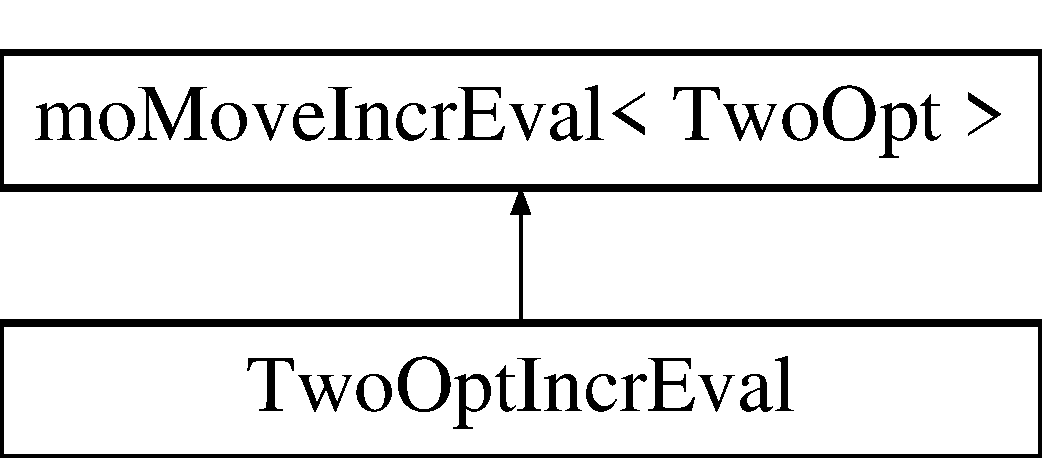
\includegraphics[height=4cm]{classTwoOptIncrEval}
\end{center}
\end{figure}
\subsection*{Public Member Functions}
\begin{CompactItemize}
\item 
\hypertarget{classTwoOptIncrEval_48500077e651c4c6152daef8a396be39}{
int \hyperlink{classTwoOptIncrEval_48500077e651c4c6152daef8a396be39}{operator()} (const \hyperlink{classTwoOpt}{Two\-Opt} \&\_\-\_\-move, const \bf{Route} \&\_\-\_\-route)}
\label{classTwoOptIncrEval_48500077e651c4c6152daef8a396be39}

\end{CompactItemize}


\subsection{Detailed Description}




Definition at line 43 of file two\_\-opt\_\-incr\_\-eval.h.

The documentation for this class was generated from the following files:\begin{CompactItemize}
\item 
two\_\-opt\_\-incr\_\-eval.h\item 
two\_\-opt\_\-incr\_\-eval.cpp\end{CompactItemize}

\hypertarget{classTwoOptInit}{
\section{Two\-Opt\-Init Class Reference}
\label{classTwoOptInit}\index{TwoOptInit@{TwoOptInit}}
}
\subsection*{Public Member Functions}
\begin{CompactItemize}
\item 
\hypertarget{classTwoOptInit_5bf6af064d37ebd955ffb5a623e78e1b}{
void \hyperlink{classTwoOptInit_5bf6af064d37ebd955ffb5a623e78e1b}{operator()} (\hyperlink{classTwoOpt}{Two\-Opt} \&\_\-\_\-move, const Route \&\_\-\_\-route)}
\label{classTwoOptInit_5bf6af064d37ebd955ffb5a623e78e1b}

\end{CompactItemize}


\subsection{Detailed Description}




Definition at line 32 of file two\_\-opt\_\-init.h.

The documentation for this class was generated from the following files:\begin{CompactItemize}
\item 
two\_\-opt\_\-init.h\item 
two\_\-opt\_\-init.cpp\end{CompactItemize}

\hypertarget{classTwoOptNext}{
\section{Two\-Opt\-Next Class Reference}
\label{classTwoOptNext}\index{TwoOptNext@{TwoOptNext}}
}
Inheritance diagram for Two\-Opt\-Next::\begin{figure}[H]
\begin{center}
\leavevmode
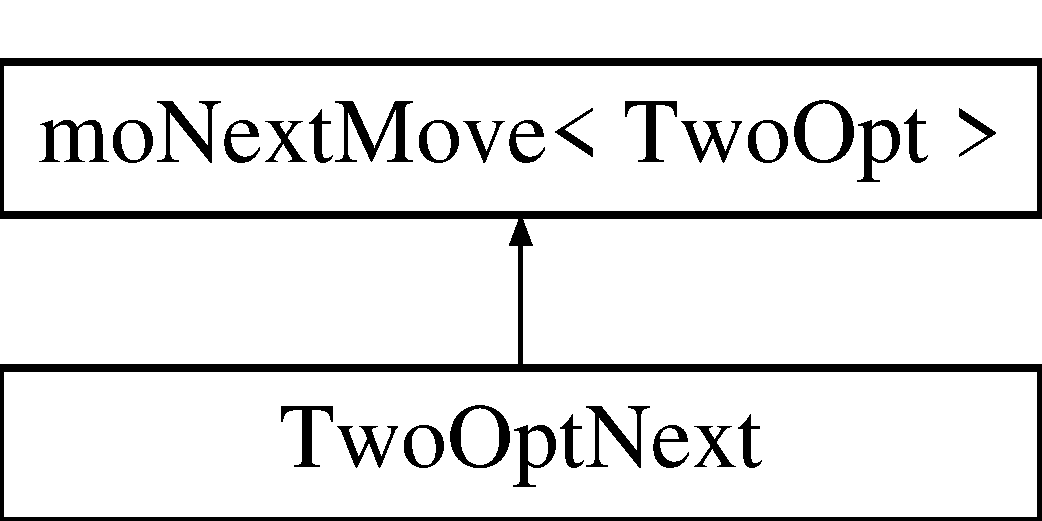
\includegraphics[height=4cm]{classTwoOptNext}
\end{center}
\end{figure}
\subsection*{Public Member Functions}
\begin{CompactItemize}
\item 
\hypertarget{classTwoOptNext_baf229b2e056f39ab971cf2ac66a833e}{
bool \hyperlink{classTwoOptNext_baf229b2e056f39ab971cf2ac66a833e}{operator()} (\hyperlink{classTwoOpt}{Two\-Opt} \&\_\-\_\-move, const \bf{Route} \&\_\-\_\-route)}
\label{classTwoOptNext_baf229b2e056f39ab971cf2ac66a833e}

\end{CompactItemize}


\subsection{Detailed Description}




Definition at line 44 of file two\_\-opt\_\-next.h.

The documentation for this class was generated from the following files:\begin{CompactItemize}
\item 
two\_\-opt\_\-next.h\item 
two\_\-opt\_\-next.cpp\end{CompactItemize}

\hypertarget{classTwoOptRand}{
\section{Two\-Opt\-Rand Class Reference}
\label{classTwoOptRand}\index{TwoOptRand@{TwoOptRand}}
}
\subsection*{Public Member Functions}
\begin{CompactItemize}
\item 
\hypertarget{classTwoOptRand_e2f362f359517c027f6f22fba0aab375}{
void \hyperlink{classTwoOptRand_e2f362f359517c027f6f22fba0aab375}{operator()} (\hyperlink{classTwoOpt}{Two\-Opt} \&\_\-\_\-move, const Route \&\_\-\_\-route)}
\label{classTwoOptRand_e2f362f359517c027f6f22fba0aab375}

\end{CompactItemize}


\subsection{Detailed Description}




Definition at line 16 of file two\_\-opt\_\-rand.h.

The documentation for this class was generated from the following files:\begin{CompactItemize}
\item 
two\_\-opt\_\-rand.h\item 
two\_\-opt\_\-rand.cpp\end{CompactItemize}

\printindex
\end{document}
